% These are the lecture notes for my CSCI360 course SPRING 2017
% at John Jay College of Criminal Justice. They are based largely on
% Schneier's Applied Cryptography.

% Feel free to edit these slides and use them for your own courses.
% HOWEVER DO NOT REMOVE THESE LINES!
% Email me at: awood [at] jjay.cuny.edu
% or at: awood [at] gradcenter.cuny.edu


\documentclass{beamer}

\usepackage{tikz}
\usetikzlibrary{calc}

\usepackage{forest}
\usepackage{verbatim}
\usepackage{color}


\setbeamertemplate{footline}[frame number]
\setbeamertemplate{navigation symbols}{} 

\newtheorem{thm}{Theorem}[section]
\newtheorem{lem}{Lemma}
\newtheorem{cl}{Claim}
\newtheorem{cor}{Corollary}[section]
\newtheorem{conj}{Conjecture}
\newtheorem{quest}{Question}
\newtheorem{defn}{Definition}[section]
\newtheorem{obs}{Observation}[section]
\newtheorem{exam}{Example}

\newcommand{\im}{\operatorname{im}}
\newcommand{\id}{\operatorname{id}}
\newcommand{\interior}{\operatorname{int}}
\newcommand{\bdry}{\operatorname{bdry}}
\newcommand{\<}{\langle}
\renewcommand{\>}{\rangle}
\newcommand{\Gab}{(G_\phi)^{ab}} 
\newcommand{\phibar}{\bar{\phi}}
\newcommand{\Z}{\mathbb{Z}}
\newcommand{\N}{\mathbb{N}}
\newcommand{\Q}{\mathbb{Q}}
\newcommand{\R}{\mathbb{R}}
\newcommand{\C}{\mathbb{C}}
\newcommand{\A}{\mathcal{A}}
\newcommand{\OO}{\mathcal{O}}
\newcommand{\UU}{\mathcal{U}}
\newcommand{\power}{2^{\{P_1, \cdots , P_n\}}}
\newcommand{\bp}{\begin{problem}}
\newcommand{\ep}{\end{problem}}
\newcommand{\ba}{\begin{answer}}
\newcommand{\ea}{\end{answer}}
\newcommand{\ds}{\displaystyle}
\newcommand{\ben}{\renewcommand{\theenumi}{\alph{enumi}}
\renewcommand{\labelenumi}{(\theenumi)}\begin{enumerate}}
\newcommand{\een}{\end{enumerate}}
\newcommand{\Hess}{\operatorname{Hessian}}
\newcommand{\Aut}{\mathrm{Aut}}
\newcommand{\Inn}{\mathrm{Inn}}
\newcommand{\Out}{\mathrm{Out}}
\newcommand{\End}{\mathrm{End}}


\mode<presentation>
{
%  \usetheme{default}
  \setbeamercovered{invisible}
}


\usepackage[english]{babel}
\usepackage[latin1]{inputenc}
\usepackage{times}
\usepackage[T1]{fontenc}
\usepackage{stmaryrd}

%\usetheme{default}
%\usetheme{AnnArbor}
%\usetheme{Antibes}
%\usetheme{Bergen}
%\usetheme{Berkeley}
%\usetheme{Berlin}
%\usetheme{Boadilla}
%\usetheme{CambridgeUS}
%\usetheme{Copenhagen}
%\usetheme{Darmstadt}
%\usetheme{Dresden}
%\usetheme{Frankfurt}
%\usetheme{Goettingen}
%\usetheme{Hannover}
%\usetheme{Ilmenau}
%\usetheme{JuanLesPins}
%\usetheme{Luebeck}
%\usetheme{Madrid}
%\usetheme{Malmoe}
%\usetheme{Marburg}
%\usetheme{Montpellier}
%\usetheme{PaloAlto}
%\usetheme{Pittsburgh}
%\usetheme{Rochester}
\usetheme{Singapore}
%\usetheme{Szeged}
%\usetheme{Warsaw}

%\usecolortheme{default}
%\usecolortheme{albatross}
\usecolortheme{beaver}
%\usecolortheme{beetle}
%\usecolortheme{crane}
%\usecolortheme{dolphin}
%\usecolortheme{dove} % grey, white, yellow
%\usecolortheme{fly} %grey, yellow
%\usecolortheme{lily} %white, yellow, blue
%\usecolortheme{orchid}
%\usecolortheme{rose}
%\usecolortheme{seagull}
%\usecolortheme{seahorse}
%\usecolortheme{whale}
%\usecolortheme{wolverine}

% Title page

\title[OOP]{Introduction to Cryptography}

\subtitle{Definitions and Common Terminology \\ Based on 1.1 of Schneier's \emph{Applied Cryptography}}

\author
{Lecture notes of Alexander Wood \\ \scriptsize \href{mailto:awood@jjay.cuny.edu}{awood@jjay.cuny.edu}}
\institute[JJay]{John Jay College of Criminal Justice}  

\date{}

\begin{document}

% Remove 'figure' text from figure captions 
\setbeamertemplate{caption}{\raggedright\insertcaption\par}

\begin{frame}
  \titlepage
\end{frame}

\section{The Game of Cryptography}


\begin{frame}
\frametitle{What is cryptography?}

Spend a few minutes thinking about how you would define this term. 

\begin{figure}

\includegraphics[scale=.4]{IMG/drake.jpg}
\end{figure}
\end{frame}

\begin{frame}
\frametitle{What is cryptography?}

Hopefully we have focused in on the main ideas:
\begin{itemize}
\item \pause \emph{Communication} between two (or more) parties..
\item \pause .. which is \emph{secure} ...
\item \pause ... in the presence of \emph{adversaries}.
\end{itemize}
\end{frame}


\begin{frame}
\frametitle{What is Cryptography?}

\emph{Cryptography} is secure communication between two or more parties in the presence of adversaries. 
\end{frame}



\begin{frame}
\frametitle{Who are the players?}

\begin{itemize}
\item The \textbf{sender} wishes to send a message.
\item The \textbf{receiver} is the intended recepient of the message.
\item The \textbf{adversary} is a malicious third party who wishes to obtain (at least partial) information about the message. 
\end{itemize}
\end{frame}

\begin{frame}
\frametitle{The Basic Setup}

\begin{figure}
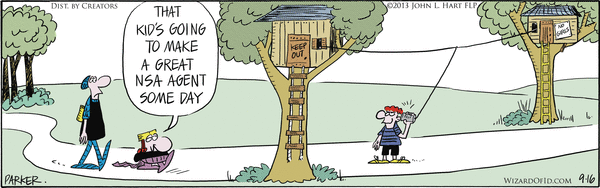
\includegraphics[scale=.5]{IMG/comic1.png}
\caption{\url{}}
\end{figure}
\end{frame}

\begin{frame}
\frametitle{The Basic Setup}

\begin{figure}
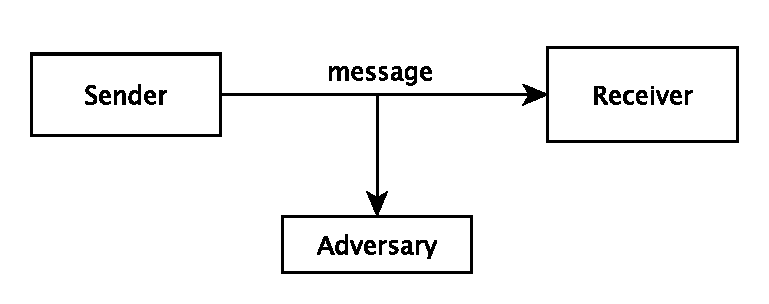
\includegraphics[scale=.8]{IMG/diag1.pdf}
\end{figure}

Let's give names to our players.
\end{frame}

\begin{frame}
\frametitle{The Basic Setup}

\begin{figure}
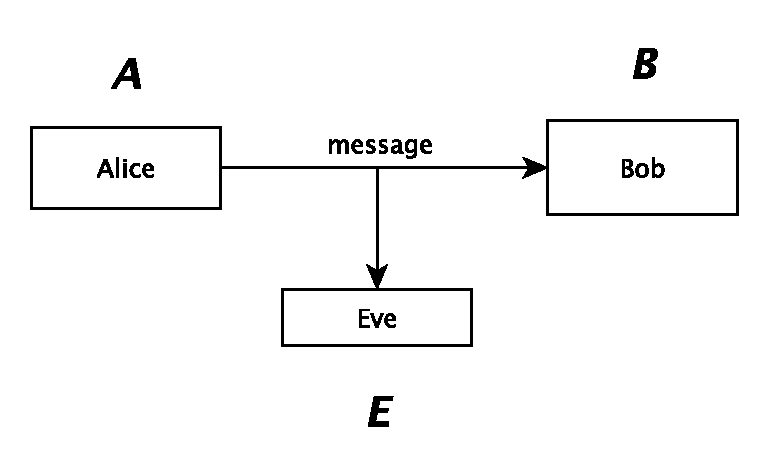
\includegraphics[scale=.8]{IMG/diag2.pdf}
\end{figure}
\end{frame}



\begin{frame}
\frametitle{Alice, Bob, and Eve}

\begin{figure}
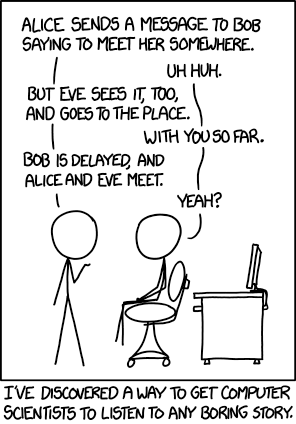
\includegraphics[scale=.5]{IMG/comic2.png}
\end{figure}
\end{frame}


\begin{frame}
\frametitle{The Basic Setup}

\begin{figure}
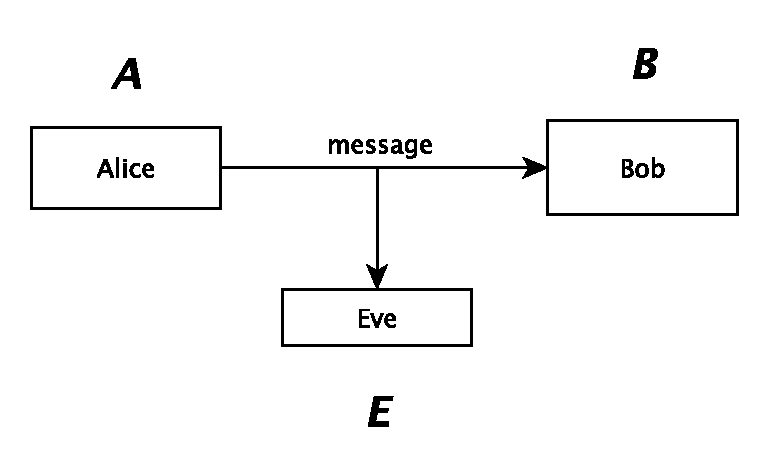
\includegraphics[scale=.8]{IMG/diag2.pdf}
\end{figure}


Observe that we have not yet introduced any way of \emph{encrypting} the message.
\end{frame}

\begin{frame}
\frametitle{Messages \& Encryption}

\begin{itemize}
\item The message is originally in \textbf{plaintext}, which can be plainly read.
\item We hide the substance of the message using \textbf{encryption}, which yields a disguised message, or \textbf{ciphertext}.
\item Turning the ciphertext back into plaintext is called \textbf{decryption}.
\end{itemize}
\end{frame}

\begin{frame}
\frametitle{Encyption and Decryption}
\begin{figure}
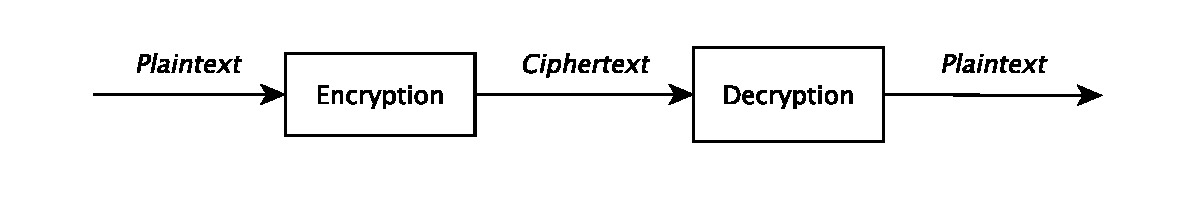
\includegraphics[scale=.5]{IMG/diag3.pdf}
\end{figure}
\end{frame}

\begin{frame}
\frametitle{An example scenario}

Alice must encrypt the message, and Bob must decrypt it. 

\begin{figure}
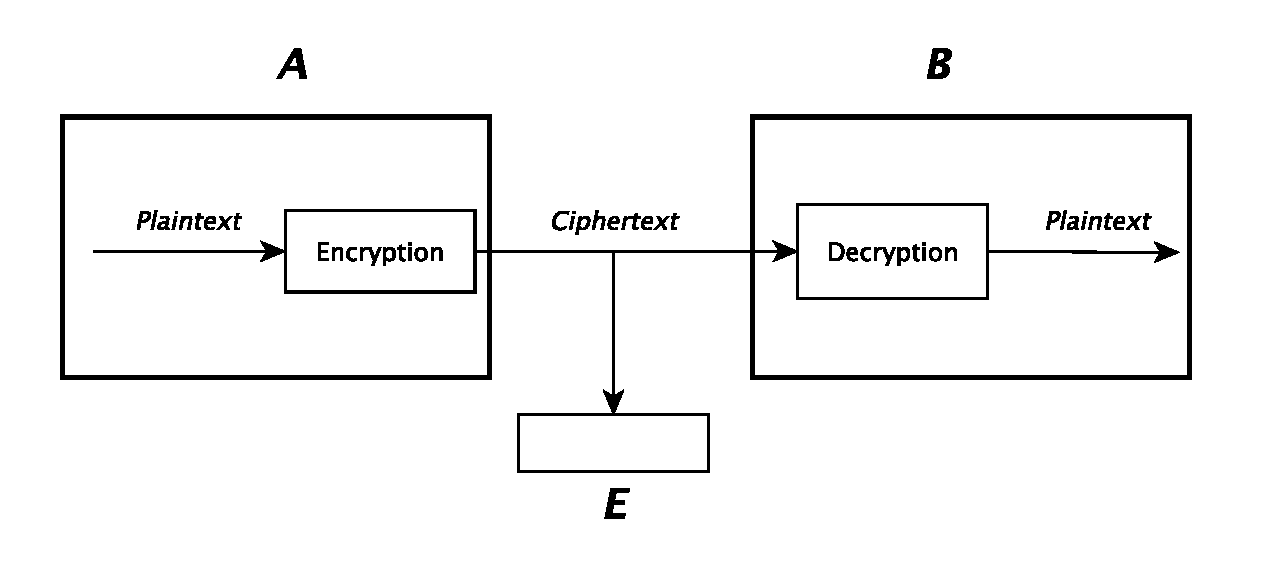
\includegraphics[scale=.5]{IMG/diag4.pdf}
\end{figure}
Note now that if Eve intercepts the message, she receives only the ciphertext. 
\end{frame}





\begin{frame}
\frametitle{Sounding Like Cryptologists (AKA, some terminology)}

\begin{itemize}
\item \textbf{Cryptography} is the science of secure communication between multiple parties, and it is practiced by \textbf{cryptographers}. 
\item \textbf{Cryptanalysis} is science of breaking ciphertext and is practiced by \textbf{cryptanalysts}.
\item Cryptography \emph{and} cryptanalysis is \textbf{cryptology} and its practitioners are \textbf{cryptologists}. 
\end{itemize}
\end{frame}

\begin{frame}
\frametitle{Naming Conventions}

\begin{itemize}
\item $M$ is the plaintext message
\item $C$ is the ciphertext, or the encrypted plaintext. 
\item $E$ or $Enc()$ represents encryption, where 
\[ 
Enc(M) = C
\]
\item $D$ or $Dec()$ represents decryption, where 
\[
Dec(C) = M
\]
\end{itemize}

We should be able to encrypt then decrypt the message to recover the original message:
\[
Dec(Enc(M)) = M
\]
\end{frame}

\begin{frame}
\frametitle{Our super cool diagram}

\begin{figure}
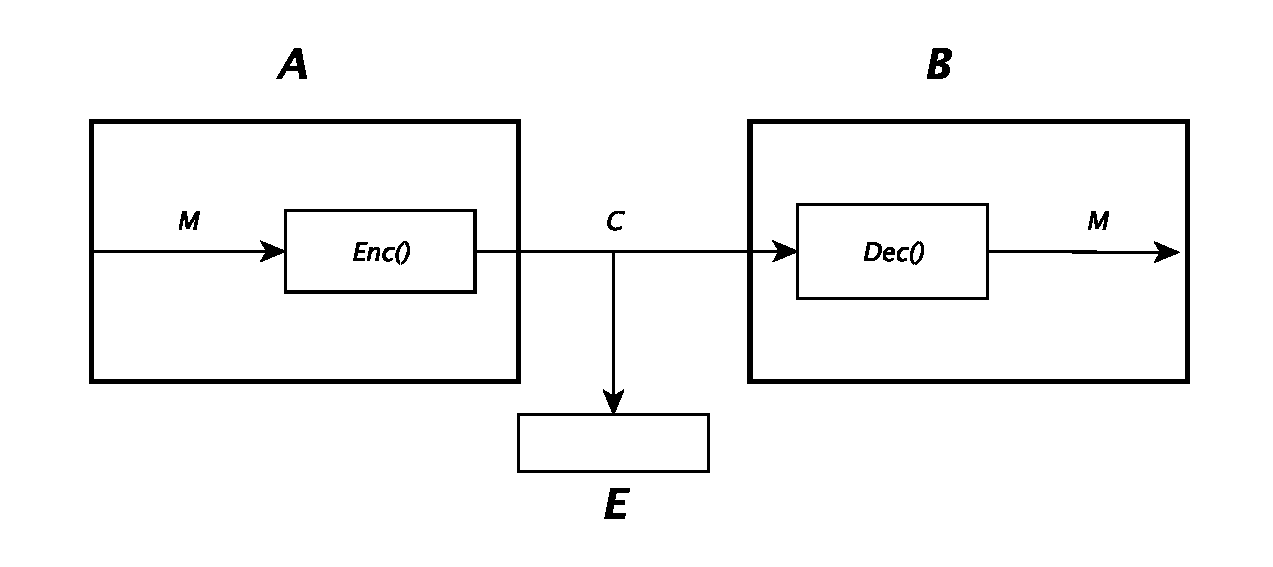
\includegraphics[scale=.5]{IMG/diag5.pdf}
\end{figure}
\end{frame}

\begin{frame}
\frametitle{But really, what's in a message?}

A plaintext message $M$  can be...

\begin{itemize}
\item A stream of bits
\item a text file
\item a digitized voice stream
\item a video
\end{itemize}

The ciphertext $C$, or encryption of the message, is binary data. It may be larger or smaller (if compressed -- discussed later in course) than the original message. 
\end{frame}





\begin{frame}
\frametitle{What else do we want from our cryptographic protocols?}

\begin{itemize}
\item Authentication
\item Integrity
\item Nonrepudiation 
\end{itemize}
\end{frame}

\begin{frame}
\frametitle{Authentication}

A third party should not be able to send a message as someone else. In other words, the receiver of a message should be able to accurately determine its origin, or authenticity. 

\begin{figure}
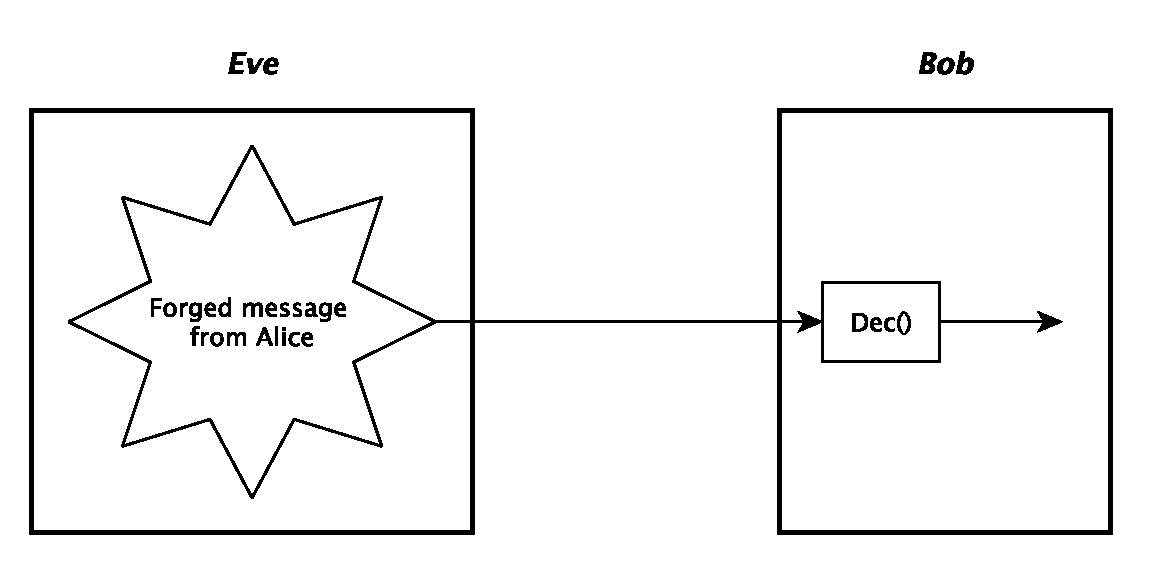
\includegraphics[scale=.5]{IMG/diag6.pdf}
\end{figure}
\end{frame}


\begin{frame}
\frametitle{Integrity}

The receiver should be able to verify that a message was not modified after being sent. 

\begin{figure}
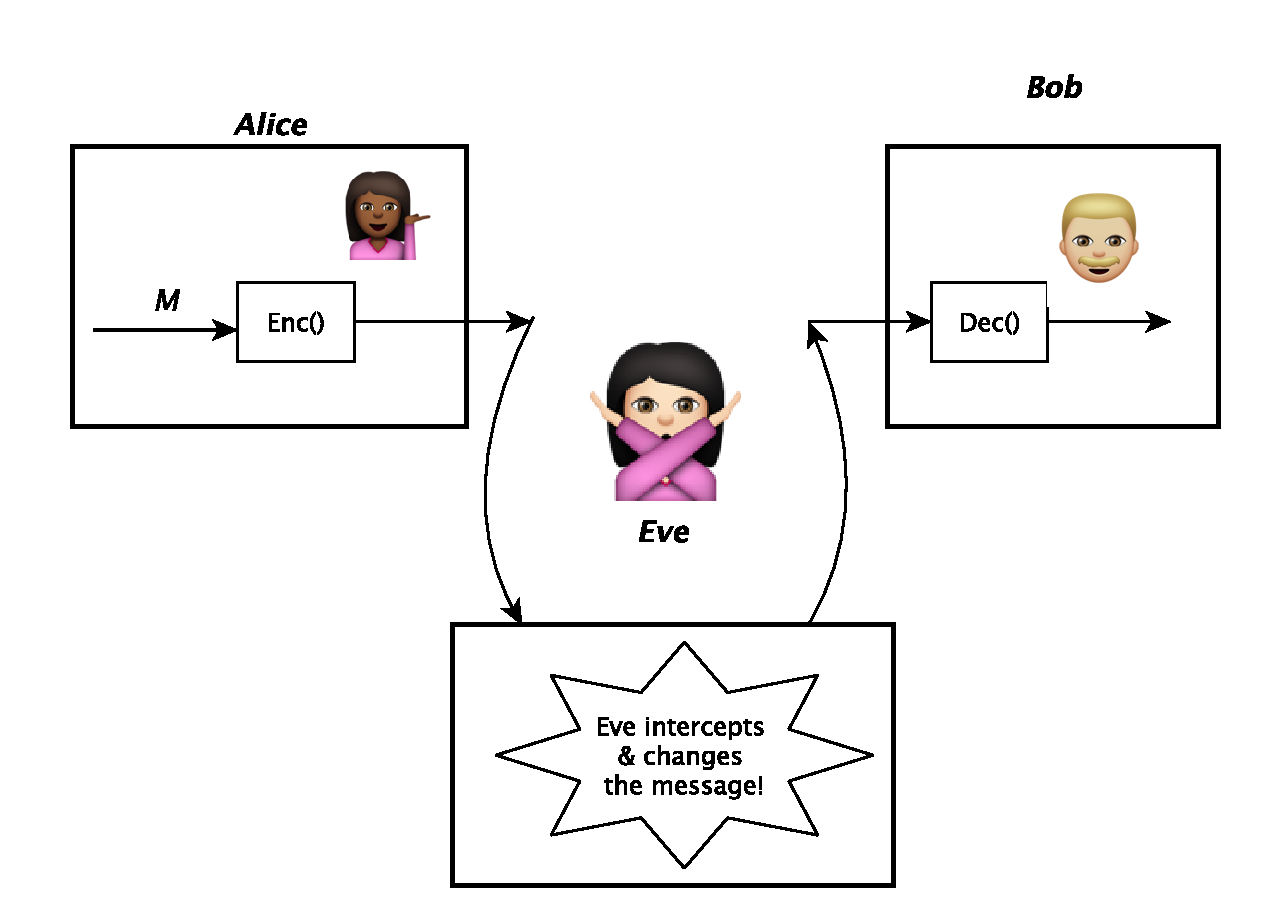
\includegraphics[scale=.4]{IMG/diag7.pdf}
\end{figure}
\end{frame}


\begin{frame}
\frametitle{Nonrepudiation}

The sender of a message cannot falsely claim to have not sent it. 

\begin{figure}

\includegraphics[scale=.2]{IMG/nonrep.jpg}
\end{figure}
\end{frame}


\begin{frame}
\frametitle{Ciphers}

A \textbf{cryptographic algorithm} is also called a \textbf{cipher}. It consists of mathematical functions for encryption and for decryption. 
\end{frame}


\begin{frame}
\frametitle{I got the keys}

\begin{figure}

\includegraphics[scale=.5]{IMG/igotkeys.png}
\end{figure}
\end{frame}


\begin{frame}
\frametitle{Keys}

Modern cryptography uses a \textbf{key} $K$, taken from a possible range of values called the \textbf{keyspace}, for encryption and decyption algorithms. Common notation for encryption and decryption under a key $K$ is given by use of a subscript:
\[
E_K(M) = C
\]

\[
D_K(C) = M
\]
\end{frame}


\begin{frame}
\frametitle{Keys}

\begin{figure}
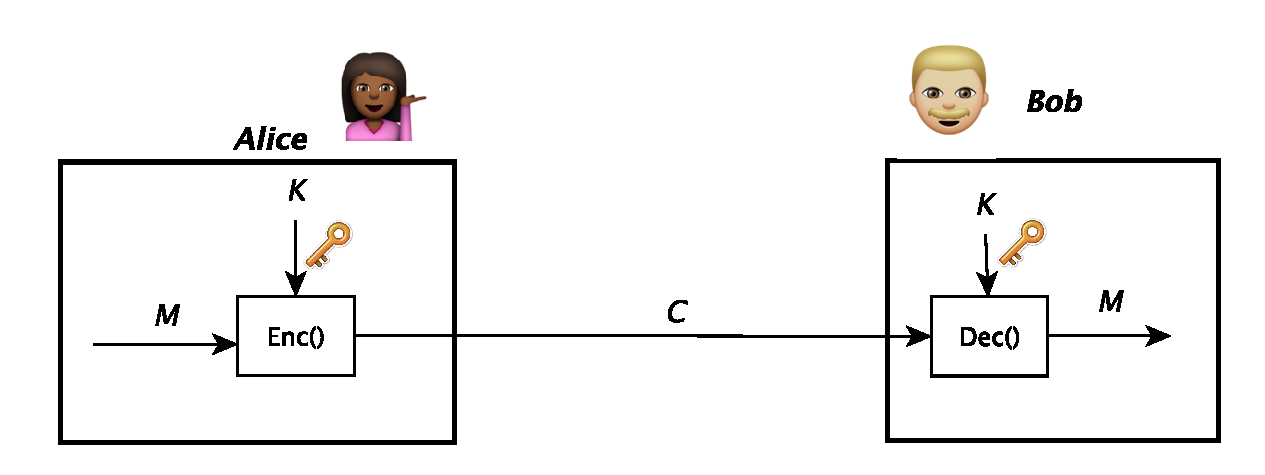
\includegraphics[scale=.5]{IMG/diag8.pdf}
\end{figure}
\end{frame}

\begin{frame}
\frametitle{Keys}

The encryption key $K$ and decryption key $\bar K$ are sometimes different.
\[
E_K(M) = C
\]

\[
D_{\bar{K}}(C) = M
\]
\end{frame}

\begin{frame}
\frametitle{Cryptosystem}

The term \textbf{cryptosystem} describes the encryption and decryption algorithms, as well as all possible plaintexts, ciphertexts, and keys. 
\end{frame}


\section{Symmetric Vs. Asymmetric} 


\begin{frame}
\frametitle{Public versus Private}

There are two main types of algorithms used in cryptosystems

\begin{itemize}
\item \textbf{Private-key}, or \textbf{symmetric} algorithms
\item \textbf{Public-key}, or \textbf{asymmetric} algorithms
\end{itemize}
\end{frame}



\begin{frame}
\frametitle{Symmetric Encryption}

These were the first types of encryption algorithms created! The encyption and decryption keys are usually the same, and they must be agreed upon \emph{beforehand} by all involved parties. 

\begin{figure}
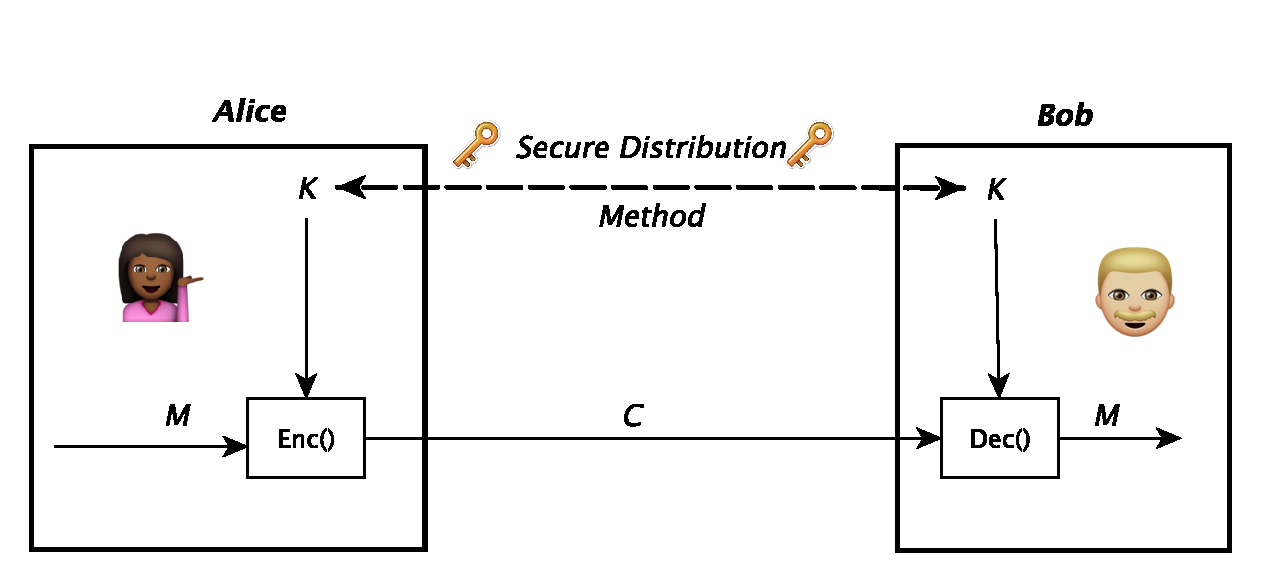
\includegraphics[scale=.5]{IMG/diag9.pdf}
\end{figure}
\end{frame}



\begin{frame}
\frametitle{Public Key Encryption}

Revolutionized by the publication of Diffie-Hellman Key Exchange in 1974. In asymmetric or public key schemes, it is not necessary to agree on a key beforehand. 
\end{frame}


\begin{frame}
\frametitle{Public Key Encryption}

Now, Bob has both a public key, which he shares publicly, and a private key, which he tells no one. Anyone can send Bob and encrypted message using his public key, but only Bob can decrypt it.
\end{frame}


\begin{frame}
\frametitle{Public Key Encryption}

\begin{figure}
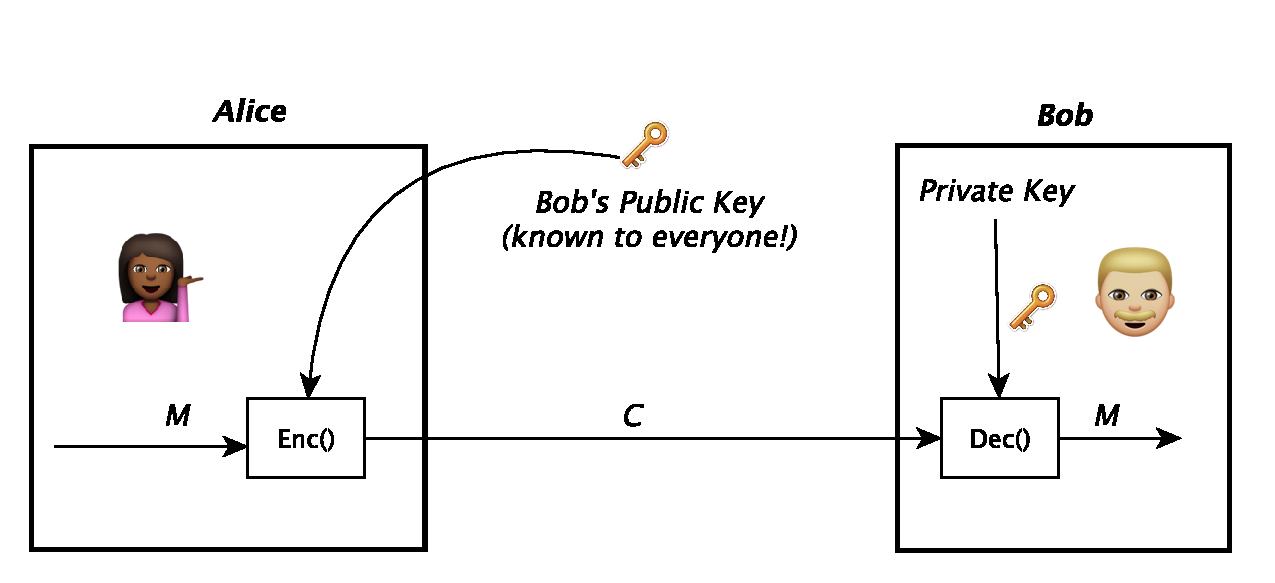
\includegraphics[scale=.5]{IMG/diag10.pdf}
\end{figure}

First, Bob publishes his public key. Then, Alice encrypts a plaintext message using this public key and sends it to Bob. Bob uses his private key and the decryption algorithm to decrypt the message.
\end{frame}

\section{Cryptanalysis}

\begin{frame}
\frametitle{Cryptanalysis}

Cryptanalysis is the attempt to recover an encrypted message without access to the key, and to find weaknesses in the cryptosystem. Call an attemped cryptanalysis an \textbf{attack} on the cryptosystem. 
\end{frame}

\begin{frame}
\frametitle{Kerckhoffs' Principle}

In the 1880s, Dutch mathematician Kerckhoff published several design principles for cryptographic algorithms. \newline

One of these, which we still follow to this day, states that even an adversary who has all of the information about how your cryptosystem operates, but does not have the private keys, will not be able to break your cryptosystem. \newline

In other words, \emph{we should be able to publish all of the information about how the cryptosystem works without compromising its security.}
\end{frame}

\begin{frame}
\frametitle{Cryptanalytic Attacks}

There are many! 

\begin{itemize}
\item Ciphertext-Only Attack
\item Known-Plaintext Attack
\item Chosen-Plaintext Attack
\item Adaptive-Chosen-Plaintext Attack
\item Chosen-Ciphertext Attack
\item Rubber-hose Cryptanalysis
\end{itemize}
\end{frame}


\begin{frame}
\frametitle{Ciphertext-Only Attacks}

\begin{itemize}
\item \emph{Given}: Ciphertexts $C_1$, $C_2$, $\dots, C_k$
\item \emph{Deduce:} $M_1$, $M_2, \dots, M_k$ or $Enc()$.
\end{itemize}

The cryptanalyst Eve eavesdropped on communication between Alice and Bob and has the ciphertext of several messages. She attempts to use properties of these plaintexts to deduce either the contents of the messages, the keys, or both. 
\end{frame}


\begin{frame}
\frametitle{Ciphertext-Only Attacks}

Eve determines they key(s) or the plaintext(s) by analyzing intercepted ciphertexts.

\begin{figure}
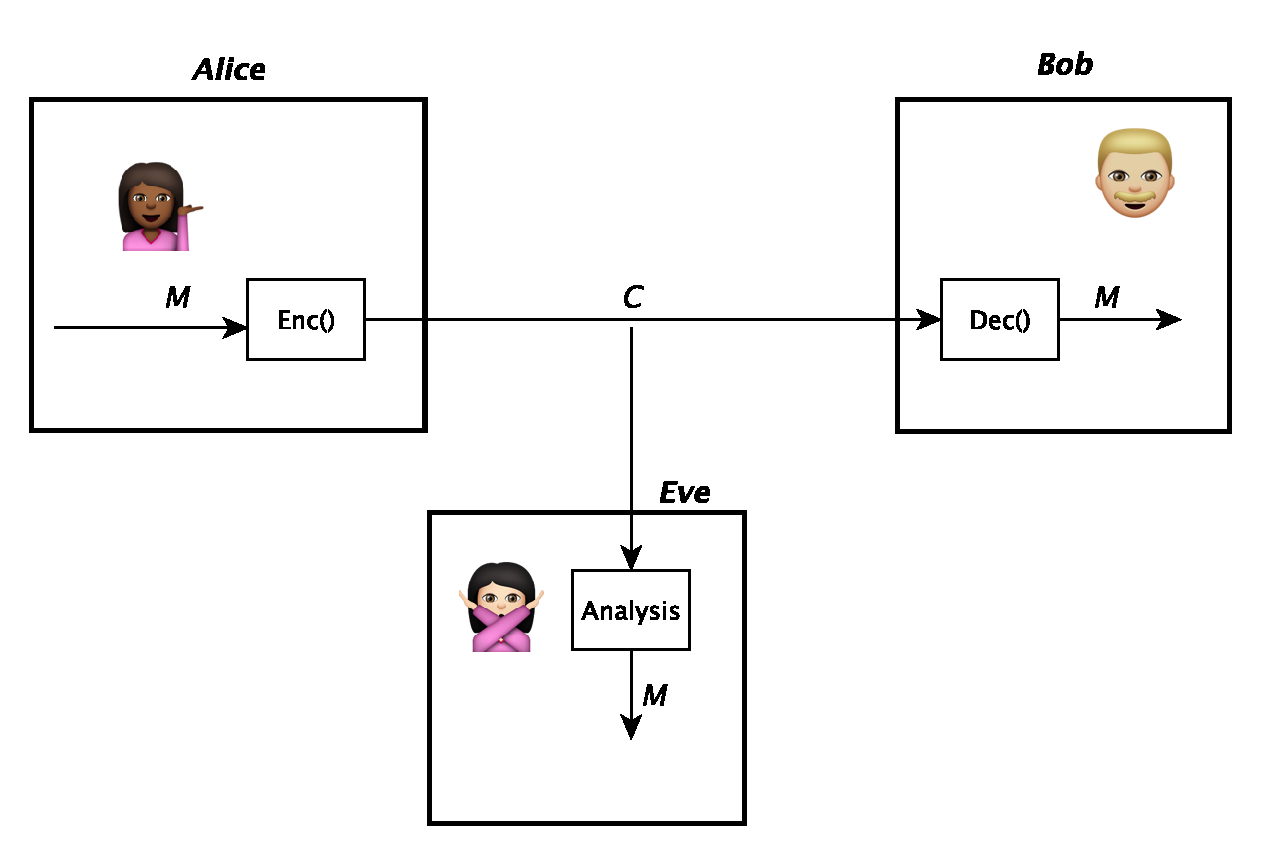
\includegraphics[scale=.4]{IMG/attack1.pdf}
\end{figure}
\end{frame}


\begin{frame}
\frametitle{Known-Plaintext Attack}

\begin{itemize}
\item \emph{Given:} Plaintexts and their associated ciphertexts
\item \emph{Deduce:} Keys and/or a method of deducing plaintexts from ciphertexts

Now, Eve not only as access to the ciphertext of several messages, but also their corresponding plaintexts. She must deduce the key(s) to the algorithm, or a method of obtaining the plaintexts from ciphertexts.
\end{itemize}
\end{frame}

\begin{frame}
\frametitle{Known-Plaintext Attack}

\begin{figure}
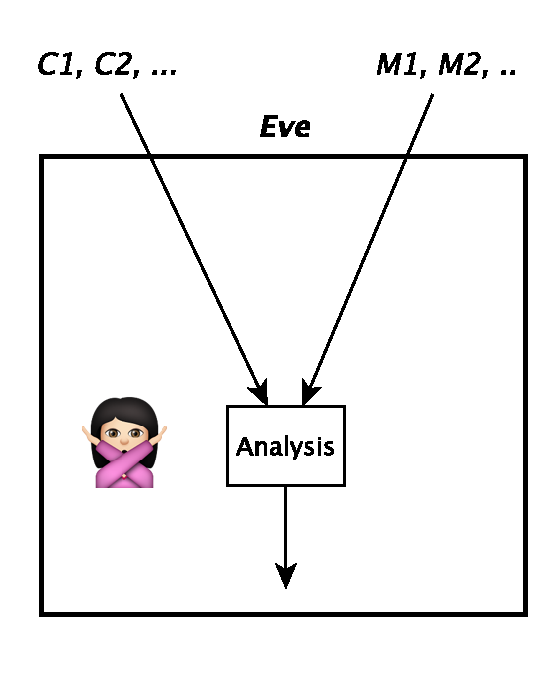
\includegraphics[scale=.4]{IMG/attack2.pdf}
\end{figure}

Eve deduces information about the cryptosytem using intercepted ciphertexts and their corresponding plaintexts. 
\end{frame}

\begin{frame}
\frametitle{Chosen-Plaintext Attack}

Eve has access to plaintexts and their corresponding ciphertexts, as before. However in a chosen-plaintext attack, Eve gets to choose which plaintexts to encrypt!
\end{frame}

\begin{frame}
\frametitle{Chosen plaintext attack}
\begin{columns}
\column{0.38\linewidth}
\centering
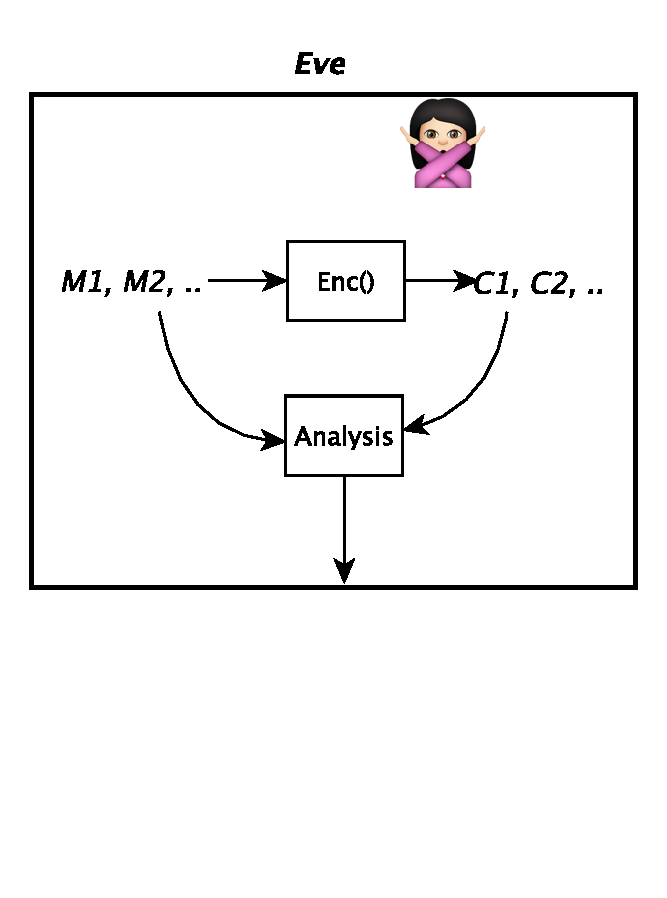
\includegraphics[scale=.5]{IMG/attack2half.pdf}
\column{0.3\linewidth}
Eve chooses which plaintexts to encrypt. \newline

What happens if a public-key cryptosystem is vulnerable to this attack?
\end{columns} 
\end{frame}



\begin{frame}
\frametitle{Adaptive-Chosen-Plaintext Attack}

\begin{columns}
\column{0.38\linewidth}
\centering
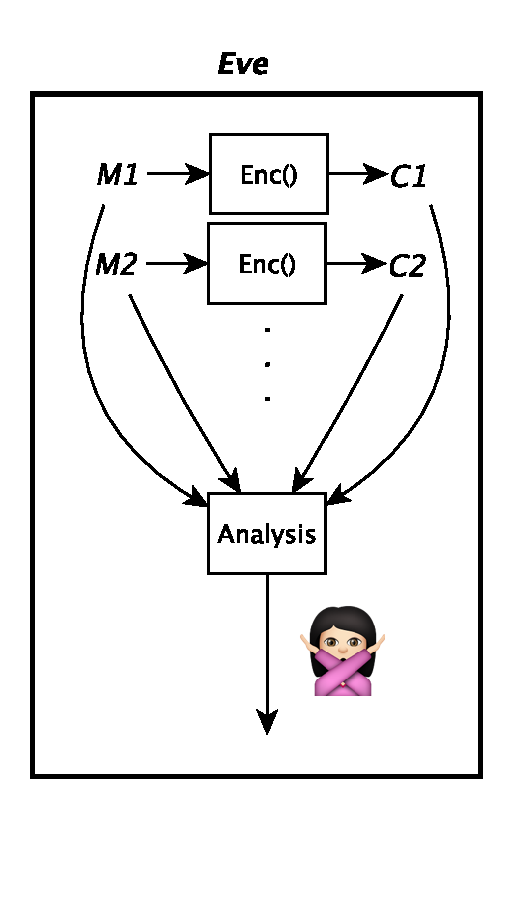
\includegraphics[scale=.5]{IMG/attack3.pdf}
\column{.58\linewidth}
This is similar to the previous attack. However, before, Eve had to choose all of the plaintexts she would like to encrypt up front. Now, Eve can adapt the plaintexts she encrypts based off of previous encryptions. \newline

What happens if a public-key cryptosystem is vulnerable to this attack?
\end{columns} 
\end{frame}

\begin{frame}
\frametitle{Chosen Ciphertext Attack}

\begin{itemize}
\item \emph{Given:} $C_1, M_1 = D_K(C_1), \dots, M_i = D_K(C_i)$
\item \emph{Deduce:} $K$
\end{itemize}

This attack is most relevant for public-key encryption. Eve can choose any ciphertexts to be decrypted, and is able to access their decrypted plaintexts. 
\end{frame}

\begin{frame}
\frametitle{Chosen Ciphertext Attack}
\centering
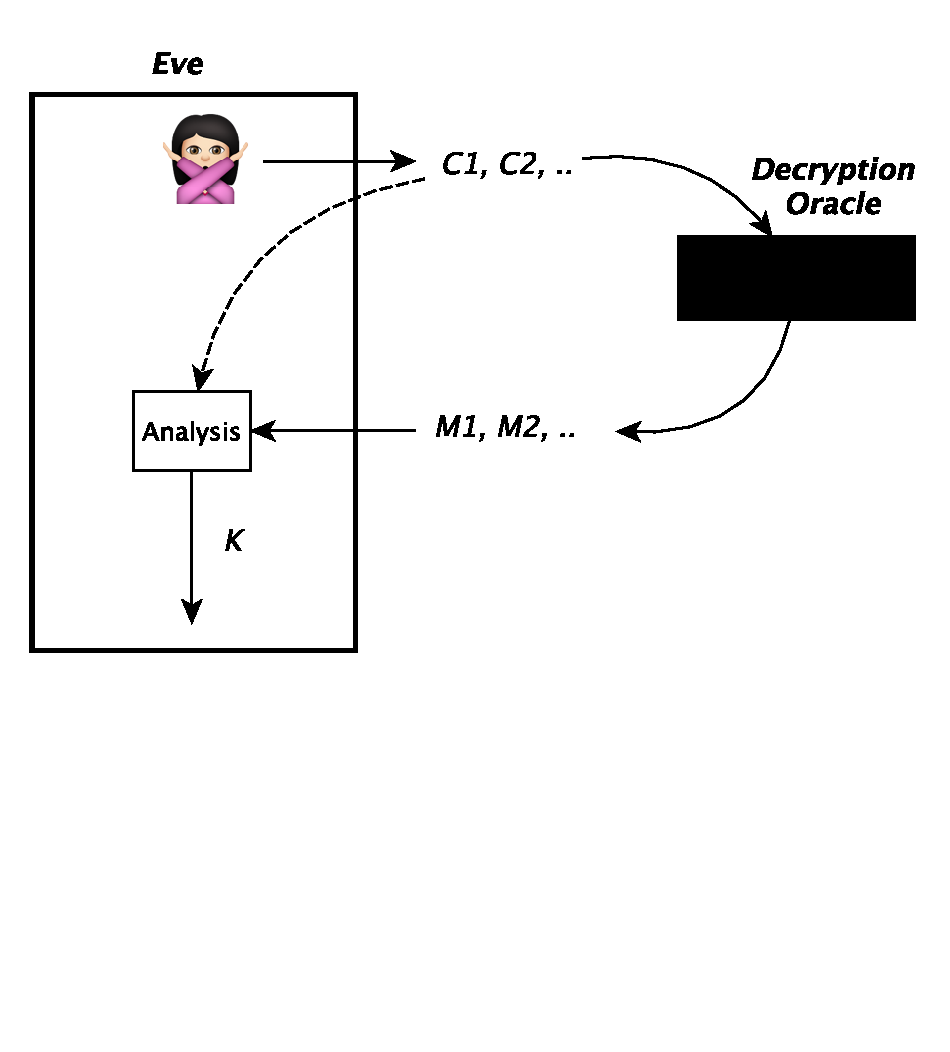
\includegraphics[scale=.5]{IMG/attack4.pdf}
\end{frame}


\begin{frame}
\frametitle{Rubber Hose Cryptanalysis}

Threaten/blackmail/torture the keyholder until they give you the key. 

\begin{figure}
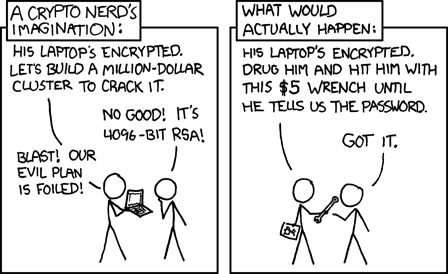
\includegraphics[scale=.5]{IMG/comic3.png}
\caption{\url{https://xkcd.com/538/}}
\end{figure}
\end{frame}


\section{Security}

\begin{frame}
\frametitle{Security}

There are many ways to define security. The definition of security we use must correspond to the cryptosystem we are using, as well as the context in which we use that scheme.  \newline

What do you think are some of the key points that must be addressed by a definiton of security?
\end{frame}

\begin{frame}
\frametitle{Security}

It should be impossible for the attacker to...
\begin{itemize}
\item ...recover the key..
\item ...recover the entire plaintext from the ciphertext...
\item ...recover part of the plaintext from the cipher text, and 
\item the ciphertext leaks no additional information about the underlying plaintext.
\end{itemize}

These are still not precisely defined terms. We will see various definitions of security throughout the course. \newline

\tiny (From \emph{Introduction to Modern Cryptography}  by Katz \& Lindell)
\end{frame}

\begin{frame}
\frametitle{Security}

You are probably safe if... 
\begin{itemize}
\item ... the cost of breaking an algorithm is greater than the value of the encrypted data...
\item ... or if the time it would take to break the algorithm is longer than then amount of time the data must remain secret.
\end{itemize}

We will see definitions of security later in the course built around these concepts.
\end{frame}

\begin{frame}
\frametitle{Unconditional Security}

We call an algorithm unconditionally secure if no amount of time and/or computational power would be enough for any adversary to ever recover the plaintext. The only unconditionally secure cryptosystem is the \textbf{one-time pad} which we will see later in this course.
\end{frame}

\begin{frame}
\frametitle{Brute-Force Attacks}

All other cryptosystems could be broken by a ciphertext-only attack. The attacker would simply have to try every possible key until she found the correct one. This is called a \textbf{brute-force attack.}\newline

A cryptosystem is called \textbf{computationally secure} if it is unfeasible to break the system with current and foreseeable future computational resources. 
\end{frame}

\begin{frame}
\frametitle{Example From Textbook}

If an algorithm has a processing complexity of $2^{128}$, then $2^{128}$ operations are required to break the algorithm. (These operations may be complex and time-consuming.) Still, if you assume that you have enough computing speed to perform a million operations every second and you set a million parallel processors against the task, it will still take over $10^{19}$ years to recover the key. That's a billion times the age of the universe.
\end{frame}
\end{document}


